\chapter{Iterators}

\section{Introduction to Iteration in Rust}
In imperative programming, the classic way to traverse a collection is by using index-based \texttt{for} or \texttt{while} loops. While functional, manual indexing presents several issues: it is prone to off-by-one errors, relies heavily on the specific memory layout of the collection (e.g., contiguous arrays), and can be inefficient or unwieldy for complex data structures like trees or linked lists.

Rust solves this uniformly through \textbf{Iterators}. An iterator is an object that logically points to elements in a collection and provides a safe, consistent interface to traverse them, without exposing the underlying implementation details of the data structure.

\begin{insightbox}
\textbf{The Water Pipe Analogy} \\
Rust iterators are \textit{lazy}. You can think of an iterator pipeline as a complex plumbing system of pipes, filters, and valves. Setting up the pipeline (chaining iterator methods) does absolutely nothing on its own—no water flows. It is only when you open the faucet at the very end (by calling a \textit{consumer} method) that the water begins to flow through the system, pulling elements one by one from the source.
\end{insightbox}

\section{The \texttt{Iterator} Trait}
At the heart of Rust's iteration model is the \texttt{Iterator} trait. Unlike some languages that require both \texttt{hasNext()} and \texttt{next()} methods, Rust elegantly condenses this into a single \texttt{next} method that returns an \texttt{Option}.

\begin{lstlisting}[language=Rust]
pub trait Iterator {
    type Item; // The type of the elements being iterated over

    fn next(&mut self) -> Option<Self::Item>;
    
    // ... plus dozens of default methods (adapters and consumers)
}
\end{lstlisting}

When \texttt{next()} is called, it returns \texttt{Some(value)} if there is another element available. Once the source is exhausted, it returns \texttt{None}. Subsequent calls after \texttt{None} is returned will typically continue to return \texttt{None}.

\begin{notebox}
\textbf{Associated Types} \\
The \texttt{Iterator} trait uses an \textit{associated type} (\texttt{type Item;}) rather than a generic parameter (\texttt{Iterator<T>}). This design choice ensures that there is exactly one implementation of \texttt{Iterator} for a given type, meaning the compiler always unambiguously knows what type an iterator will yield.
\end{notebox}

\section{Obtaining Iterators: \texttt{IntoIterator}}
To use a \texttt{for} loop over a collection, the collection must implement the \texttt{IntoIterator} trait, which tells the compiler how to convert the collection into an iterator. 

Under the hood, a \texttt{for} loop is syntactic sugar for a \texttt{while let} loop that continuously calls \texttt{next()}:

\begin{lstlisting}[language=Rust]
// What you write:
for x in vec {
    println!("{}", x);
}

// What the compiler sees:
let mut it = vec.into_iter();
while let Some(x) = it.next() {
    println!("{}", x);
}
\end{lstlisting}

Standard collections generally offer three distinct ways to create an iterator, dictating how the elements are yielded:

\begin{enumerate}
    \item \textbf{\texttt{iter()}} yields immutable references (\texttt{\&T}). The collection remains intact and owned by its original scope.
    \item \textbf{\texttt{iter\_mut()}} yields mutable references (\texttt{\&mut T}). The collection remains intact, but you can mutate its elements in place.
    \item \textbf{\texttt{into\_iter()}} yields values by taking ownership (\texttt{T}). The collection is consumed and destroyed in the process.
\end{enumerate}

\begin{warningbox}
\textbf{Implicit \texttt{into\_iter} in \texttt{for} loops} \\
If you write \texttt{for x in my\_vec}, you are implicitly calling \texttt{into\_iter()}, which consumes \texttt{my\_vec}. If you need to use the vector afterward, you must iterate over a reference instead: \texttt{for x in \&my\_vec} (which calls \texttt{iter()}).
\end{warningbox}

\section{Iterator Adapters}
Adapters are methods defined on the \texttt{Iterator} trait that consume an iterator and build a \textit{new} iterator with a modified behavior. Because iterators are lazy, adapters incur zero runtime cost until they are consumed.

Common adapters include:
\begin{itemize}
    \item \textbf{\texttt{map(f)}}: Applies a closure \texttt{f} to each element, transforming it to a new type or value.
    \item \textbf{\texttt{filter(p)}}: Applies a predicate closure \texttt{p}. Only elements for which the predicate returns \texttt{true} are yielded.
    \item \textbf{\texttt{enumerate()}}: Yields a tuple \texttt{(index, value)}, giving you the iteration count alongside the element.
    \item \textbf{\texttt{take(n)}}: Yields only the first \texttt{n} elements, then returns \texttt{None}.
    \item \textbf{\texttt{skip(n)}}: Discards the first \texttt{n} elements, yielding everything that follows.
    \item \textbf{\texttt{zip(other)}}: Zips two iterators together into a single iterator of pairs \texttt{(a, b)}. It stops as soon as the shortest iterator is exhausted.
    \item \textbf{\texttt{chain(other)}}: Appends \texttt{other} to the end of the current iterator.
\end{itemize}

\begin{figure}[htbp]
    \centering
    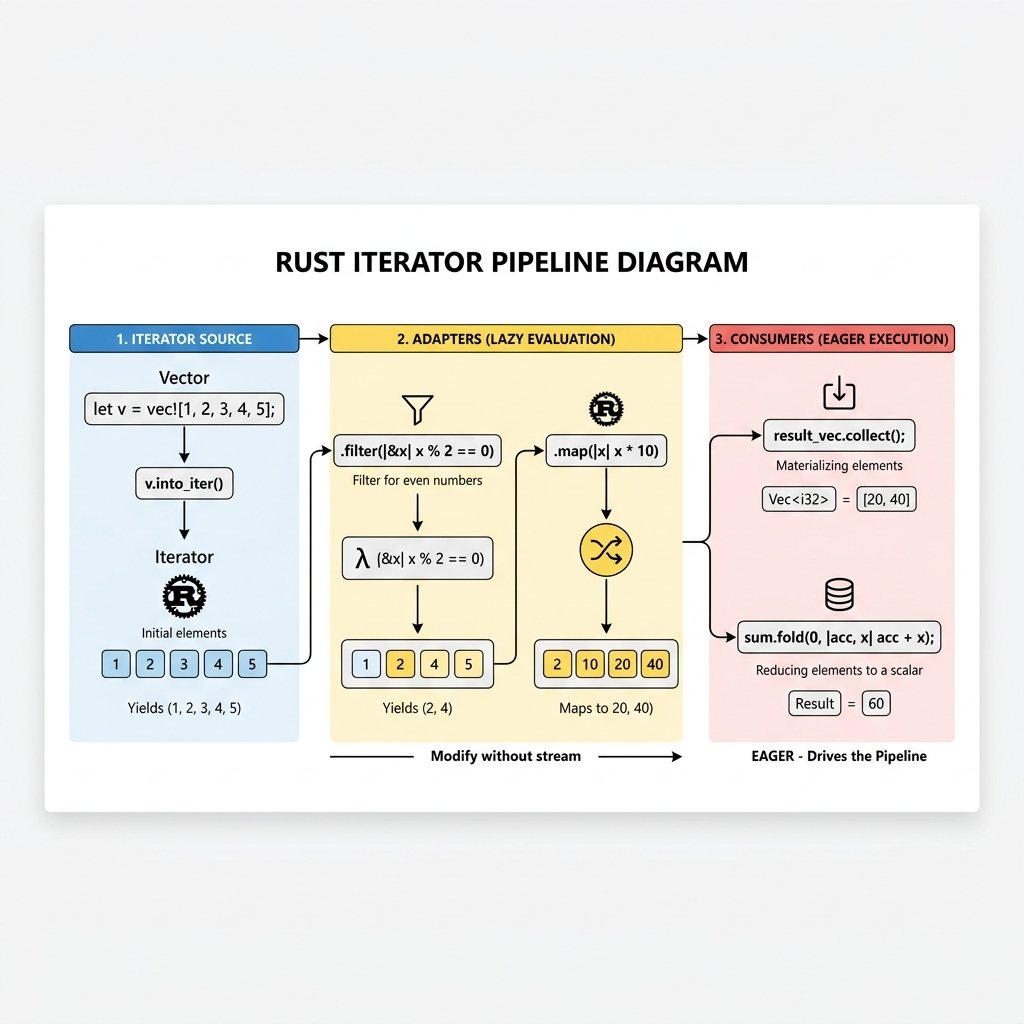
\includegraphics[width=\textwidth]{images/iterator_pipeline.png}
    \caption{A pipeline of iterator adapters lazily transforming a stream of data.}
\end{figure}

Let's look at an example combining adapters:

\begin{lstlisting}[language=Rust]
let numbers = vec![1, 2, 3, 4, 5, 6];

// The pipeline is built, but nothing is executed yet!
let pipeline = numbers.iter()
    .filter(|&&x| x % 2 == 0)   // Keep evens: 2, 4, 6
    .map(|&x| x * x);           // Square them: 4, 16, 36
\end{lstlisting}

\section{Iterator Consumers}
Consumers are methods that execute the iterator pipeline. They repeatedly call \texttt{next()} to pull elements through the adapters until \texttt{None} is reached, producing a final value or triggering side effects.

\subsection{The Universal Consumer: \texttt{fold}}
\texttt{fold} is the foundational consumer method. Almost all other consumers can be expressed in terms of \texttt{fold}. It works similarly to the accumulator register in a CPU: it starts with an initial value and repeatedly applies a closure to combine the accumulator with the next element in the iterator.

\begin{lstlisting}[language=Rust]
let numbers = vec![1, 2, 3, 4];
// sum starts at 0. 
// Step 1: acc = 0, x = 1 -> acc = 1
// Step 2: acc = 1, x = 2 -> acc = 3
// Step 3: acc = 3, x = 3 -> acc = 6
// Step 4: acc = 6, x = 4 -> acc = 10
let total = numbers.iter().fold(0, |acc, &x| acc + x);
\end{lstlisting}

\subsection{Other Common Consumers}
\begin{itemize}
    \item \textbf{\texttt{collect()}}: Gathers the yielded elements into a new collection (e.g., \texttt{Vec}, \texttt{HashMap}, \texttt{String}). You often need to provide a type hint (the "turbofish" syntax \texttt{::<>}) so the compiler knows what collection to build.
    \item \textbf{\texttt{sum()}, \texttt{product()}}: Mathematically combine numeric elements.
    \item \textbf{\texttt{count()}}: Returns the number of elements yielded.
    \item \textbf{\texttt{min()}, \texttt{max()}}: Finds the minimum or maximum element.
    \item \textbf{\texttt{any(p)}, \texttt{all(p)}}: Short-circuiting boolean evaluations based on a predicate.
\end{itemize}

\begin{exambox}
\textbf{Performance Profile of Iterators} \\
Iterators and adapters in Rust are compiled to highly optimized state machines. The compiler aggressively inlines closures and eliminates the overhead of the method calls. This means chaining \texttt{map} and \texttt{filter} is typically just as fast—and sometimes faster, due to missing bounds checks—as writing a manual \texttt{for} loop with raw indexing! This principle is known as \textbf{Zero-Cost Abstraction}.
\end{exambox}

\section{Implementing a Custom Iterator}
You can create iterators for your own types by maintaining a state and implementing the \texttt{Iterator} trait. Let's design a custom iterator that splits a string into words based on spaces, exactly as shown in lecture.

\begin{lstlisting}[language=Rust]
struct WordsIter<'a> {
    text: &'a str,
    pos: usize,
}

impl<'a> Iterator for WordsIter<'a> {
    type Item = &'a str;

    fn next(&mut self) -> Option<Self::Item> {
        let bytes = self.text.as_bytes();
        let len = bytes.len();
        
        // Skip leading spaces
        while self.pos < len && bytes[self.pos] == b' ' {
            self.pos += 1;
        }
        
        if self.pos >= len {
            return None; // Exhausted
        }
        
        let start = self.pos;
        
        // Find the end of the word
        while self.pos < len && bytes[self.pos] != b' ' {
            self.pos += 1;
        }
        
        // Return a slice of the original string
        Some(&self.text[start..self.pos])
    }
}
\end{lstlisting}

By tracking the current \texttt{pos} index and using lifetimes to tie the returned \texttt{\&str} to the source \texttt{text}, we have built an iterator that allocates zero memory, making it blazingly fast and memory-efficient.

\section*{End-of-Chapter Exam Questions}

\begin{enumerate}
    \item \textbf{Lazy Evaluation:} Explain what happens when the following code is executed. Does it panic? Why or why not?
\begin{lstlisting}[language=Rust]
let infinite_iter = 0..;
let pipeline = infinite_iter.map(|x| x / 0);
\end{lstlisting}

    \item \textbf{Ownership in Loops:} Consider a \texttt{Vec<String>} named \texttt{names}. Explain the difference between iterating with \texttt{for name in names} versus \texttt{for name in \&names}. What type is \texttt{name} in each case, and what happens to the \texttt{Vec} after the loop finishes?

    \item \textbf{Iterator Implementation:} Using the \texttt{fold} method, write a single line of code that takes an iterator of integers and returns the maximum value. Assume the iterator yields at least one positive integer. (Hint: \texttt{std::cmp::max} might be useful).
\end{enumerate}
